%%%% ijcai17.tex

\typeout{Motif-Aware Graph Embeddings}

% These are the instructions for authors for IJCAI-17.
% They are the same as the ones for IJCAI-11 with superficical wording
%   changes only.


\documentclass{article}
% The file ijcai17.sty is the style file for IJCAI-17 (same as ijcai07.sty).
\usepackage{ijcai17}
\usepackage{amsthm}
\usepackage{amssymb}
\usepackage{amsmath}
% Use the postscript times font!
\usepackage{times}
\usepackage{graphicx} 
\usepackage[ruled,vlined]{algorithm2e}
\usepackage{multicol}
\usepackage{float}

% the following package is optional:
%\usepackage{latexsym}

\DeclareMathOperator*{\argmin}{arg\,min}
\DeclareMathOperator*{\argmax}{arg\,max}


\theoremstyle{definition}
\newtheorem{definition}{Definition}[section]

\title{Motif-Aware Graph Embeddings}

\author{Anonymous authors}

\begin{document}

\maketitle

\begin{abstract}

  In this paper, we propose our motif-aware approaches to the 
  unsupervised network embedding and semi-supervised network labeling 
  task. Our first algorithm is an unsupervised network embedding 
  algorithm which uses the most statistically significant network motif 
  as the guiding pattern for random walks to generate network context. We 
  then use a Skipgram neural network to learn the latent network node 
  representations from the generated context via Noise Contrastive 
  Estimation. The second algorithm employs the Graph Convolution Network 
  model on motif Laplacian matrices to inject the higher-order network 
  structure into the neural network. Both of our algorithms utilize the 
  higher-order organization (i.e. motifs organization) of complex 
  networks. We demonstrate the effectiveness of our algorithms in 
  comparison to other state-of-the-art network embedding algorithms.

\end{abstract}

\section{Introduction}

\subsection{Complex network and machine learning}

Network modelings have been an essential tool for a wide
range of scientific fields
\cite{physicnet,molecule,youtube,motifblockmilo,juremotif}.
The network science view reveals the underlying structure 
of a complex system. Based on the system's network structure, 
scientists can make predictions and explanation
about the system's behavior. For example, in biology, the
study on neuronal systems connectivity indicated
that the component arrangement of a neural system is optimized
for short processing paths rather than wiring lengths
\cite{kaiser2006nonoptimal}. Similarly, social networks 
analysis provides communities structures well as 
social interaction patterns 
\cite{west2014exploiting,barabasi2014network}. 
However, along with the information explosion, analyzing
large network-structured datasets poses a great challenge 
for traditional network analysis methods in term of 
scalability and complexity. To deal with such challenge,
one promising approach is to apply machine learning methods 
(especially deep learning) to network problems.

Bridging the gap between network-structured data and typical
data structure for machine learning is also a challenge. 
Due to the irregularity in the network-structured data, 
it is desirable to have a \emph{meaningful}
network representation for machine learning applications. 
Learning network representation in real vector spaces can be
viewed as manifold learning (non-linear dimensionality reduction),
and commonly known as \emph{network embedding} in the literature.  
Traditionally, network embedding can be obtained via graph 
factorization methods.However, matrix factorization methods such as
Spectral Clustering or Non-negative Matrix Factorization are 
shown to be unscalable due to the complexity of the algorithms 
\cite{deepwalk,eigmaps}. Recently, several feasible network
embedding algorithms have been proposed such as \emph{Deepwalk}
\cite{deepwalk} or \emph{GCN} \cite{gcn}. These network embeddings 
algorithms utilize the state of the art machine learning models like
Skipgram \cite{Skipgram} and Variational Auto-Encoder \cite{varauto}
to achieve high quality node representation. In the context of graph
embedding, we justify the \emph{quality} by how well a common
machine learning model performs on the learned embeddings.

\begin{figure} \label{fig:cartoon}
    \centering
    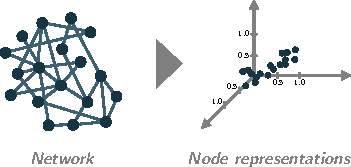
\includegraphics[width=0.8\linewidth]{cartoon_emb}
    \caption{Learning a latent representation of nodes from the network structure. In this figure, the example network is embedded to a 3-dimensional real vector space.}
\end{figure}

\subsection{Motifs in complex network}

There are three scale of network analysis: macroscopic, mesoscopic, 
and microscopic. In the macroscopic scale, we consider a network as a 
whole to study its macro-properties such as robustness 
\cite{callaway2000network}, or dynamics \cite{barabasi2014network}.
In contrast, the microscopic scale studies the pair-wise interactions
between nodes in a network which is specific to the given system 
\cite{physicnet}. In between macroscopic and microscopic, the mesoscopic 
scale considers the network is a composition of subgraphs. 
In many research, especially computational biology, the
mesoscopic components are called \emph{motifs}, and it is common
to think of them as building blocks of a complex system 
\cite{motifblockmilo}.

\begin{definition}{\emph{Network motif}}
Given a graph $G = (V,E)$, define a subgraph $G' = {V', E'}$ with $V' \subseteq V$;
$E' \subset E$ s.t. $i,j \in V' \forall e_{ij} \in E'$ and $|V'| \ll |V|$. Recurring subgraphs
are called \emph{network motif} when they are statistically significant.
\end{definition}

Also referred as higher-order organization by \citeauthor{juremotif}, 
network motifs are believed to represent the underlying mechanism of a 
complex system 
\cite{netmotif,alon2006introduction,mangan2003structure}. 
For instance, the directional bi-fan motif (figure \ref{fig:m4})
and its simplified unidirectional version are crucial in a citation 
network. Beside having a statistical significance, bi-fan motif is also 
intuitively sensible in citation network as it represents the citation 
mechanism. The correlation of recurring subgraphs and system 
functionality has been studied extensively in biological systems such as 
transcription networks \cite{mangan2003structure} and brain 
networks \cite{brainnetheuvel,honey2007network}. As networks motifs
have been recognized as the fundamental building block of a complex
systems, using them as a structural guidance for machine learning
on graph data can yield positive improvements.

In here, we propose the motif-aware approaches to improve the 
performance of  

\section{Related work}

\subsection{Unsupervised Network Embedding}

Based on the Skipgram model \cite{skipgram} in natural language 
processing, \citeauthor{Deepwalk} proposed their
scalable graph embedding algorithm named DeepWalk. Their results on node 
classification proved the effectiveness of \emph{Deepwalk} in learning a 
lower dimensionality representation of a complex network. Subsequence 
work to DeepWalk further improved node classification accuracy by 
modifying graph context generation process
\cite{line,grarep,planetoid,node2vec}. 

It is worthwhile to mention that \emph{planetoid}, proposed by 
\citeauthor{planetoid}, works slightly different to other skipgram-based 
models. Instead of generating graph context only from the network 
structure, \emph{planetoid} samples nodes based on labels as well. 
Furthermore, \emph{planetoid} injects the network
node's feature vectors for better embedding and node labeling results.

\subsection{Semi-supervised Network Labeling}

Another similar model to \emph{planetoid} called Graph Convolutional 
Networks (GCN) 
was proposed by \citeauthor{gcn}. GCN uses the graph convolutional
operation as a transformation for feature vectors on a network. By stacking
these convolutional operation into a neural network, the authors of
GCN has been able to achieve remarkable node classification and link
prediction results compared to the previous researches. Moreover, the
running time for GCN was superior compared to other algorithms.


These aforementioned approaches to graph embeddings
are similar in the sense that they all learn latent representations
of a complex network from data, then use this representation to solve 
a network problem (e.g. link prediction, node labeling, community
detection) using various machine learning algorithms.

\subsection{Motif Conductance}



Generally, algorithms involving network motifs have to deal with
the problem of graph isomorphism. For such reason, in most analysis,
only motifs of size 5 or smaller are considered. In this paper,
we only consider motif of size 4 at most. This limitation is due to
the large size of networks that we experimented. Although limited 
by the motif size, we have been able to practically show the 
effectiveness of the motif-aware methods. On the other hand, as mentioned 
in \cite{juremotif},
motif algorithms can be easily parallelized. Therefore, the extension to
larger size motifs can be made possible by parallelize the motif
analysis procedures. Further discussion will be provided in later 
sections.

\section{Methods}

In this section, we present the detail of our methods. Firstly,
we propose the basis for the network motif selection from a network.
Secondly, we present two approaches employing motif patterns to
learn graph embeddings: \emph{motifwalk} and \emph{m-gcn}.

\subsection{Motifs Adjacency Matrix}

In the previous section, we have introduced the importance of
network motifs in network analysis. In this section, we present
the metric for measuring network motif significance and the definition
of motif laplacian.

In order to measure the importance of a network motif, we compare
the given network against a null model. The null model of an empirical 
network 
is an ensemble of randomly generated networks having the same number of nodes and
edges as the network. For small networks with less than 10,000 edges, we
generated 100 random networks as the ensemble of the null model. On the other
hand, we generated 10 random networks for the null model of larger networks.
The $z\mbox{-score}$ is given by:
\begin{equation*}
z\mbox{-score} = \frac{N_\mathbf{m}(G)-N_\mathbf{m}(G_{\scalebox{0.75}{random}})}{\sigma_\mathbf{m}(G_{\scalebox{0.75}{random}})}
\end{equation*}
where $N_\mathbf{m}(G)$ is the count of motif $\mathbf{m}$ in the empirical
network; $N_\mathbf{m}(G_{\scalebox{0.75}{random}})$ is the mean of the
null model; and $\sigma_\mathbf{m}(G_{\scalebox{0.75}{random}})$ is the variance.
The $z\mbox{-score}$'s values can range from $-\inf$ to $+\inf$. In practice,
the most simple motifs (figure \ref{fig:m3}-m2,3,4) often have the highest
frequencies and negative $z\mbox{-score}$. We ignored such motifs in our analysis.
We select motif which has the highest positive $z\mbox{-score}$ and the highest frequency
as our motif of interest to construct the motif co-occurrence matrix.

\begin{definition} \emph{Motif co-occurence matrix}
Given a graph $G = (V,E)$, in which $v \in V$. The motif co-occurrence matrix
is given by:
$$M_{i,j} = \sum_{(v, \chi_{\mathcal{A}}(v)) \in \mathbf{m}} \mathbf{1}({i,j} \subset \chi_\mathcal{A}(v))$$
In here, $\mathcal{A}$ represents the anchor set; $(v, \chi_{\mathcal{A}}(v))$ 
represents pairs of node $v \in V_G$ and the other anchor nodes generated by $\chi_\mathcal{A}$.
If the anchor node set $\mathcal{A}$ is empty, all motif co-occureence is
counted toward the motif co-occurrence matrix $M$. Otherwise, only nodes in
the anchor set will be counted. Figure \ref{fig:anchor} illustrates
the bi-fan motif and its anchor set.
\end{definition}

Generally, in this paper we employ the motif co-occurrence matrix
as: 1. An adjacency matrix describing a motif graph; 2. An adjacency
matrix from which we computes the Fourier basis for the graph convolution
operation. The first approach is straight forward as we want to generate
a network context where nodes occur in the motif pattern. For such reason,
we treat the motif co-occurrence matrix as a binary matrix describing a new
network. On the other hand, the graph convolution approximation methods 
proposed in \cite{gcn,defferrard2016convolutional} only apply to symmetric 
binary matrices. In our model, the motif co-occurrence matrix is a symmetric 
weighted matrix. The eigenvalue decomposition of such matrix is given by:
\begin{equation} \label{eq:eigm}
\mathcal{L}_{\mathbf{m}} = U_{\mathbf{m}} \Lambda_{\mathbf{m}} U^{\top}_{\mathbf{m}}
\end{equation}
where $\mathcal{L}_{\mathbf{m}} = D_{\mathbf{m}} - A_{\mathbf{m}}$; $U_{\mathbf{m}}$ is the
orthogonal basis (also called the Fourier basis in graph convolutional context);
and $\Lambda_{\mathbf{m}} = diag(\lambda_{\mathbf{m}})$. 

The convolution on a graph $G$ of a function of the graph 
Laplacian $g_{\theta}$ (also called a filter or a kernel) 
and a signal $x$ is defined as:
$$g_{\theta} \ast x = U g_{\theta} U^{\top} x,$$
where $L = U \Lambda U^\top$, $U$ is the Fourier basis
and $\Lambda$ is called the frequencies of the graph. 
Graph convolution has been shown effective in processing
graph-structured data, and also argued to be the generalization
of convolutional networks
\cite{shuman2013emerging,defferrard2016convolutional,gcn}.
In practice, given a graph where each node has a feature vector,
we can treat the feature vector of the graph as signals. The output $y$
of these "signals" filtered by $g_\theta$ on the graph is given by
the graph convolution and deconvolution operations: 
\begin{equation}
\label{eq:1}
y = g_\theta (U \Lambda U^\top) x = U (g_\theta(\Lambda) U^\top)x
\end{equation}

Computing equation \ref{eq:1} is computationally expensive
due to the matrix multiplication and eigenvector decomposition operations.
Therefore, fast estimation methods such as Chebyshev polynomial was suggested
in \cite{hammond2011wavelets}.

\begin{algorithm}[h] \label{al:madj}
\KwData{Graph $G = (V,E)$}
\KwIn{isBinary, $\mathbf{m}$, $\mathcal{A}$}
\KwOut{$M^{\mathbf{m}}$}
\Begin{
    diam $\leftarrow$ Diameter($\mathbf{m}$, $\mathcal{A}$); \\
    $V$ $\leftarrow$ G.nodes(); \\
    \For{node $\in$ nodes} {
        $G'$ $\leftarrow$ induced graph from BFS(node, diam); \\
        \For{otherNode $\in$ $G'$} {
            \uIf{(node,otherNode) satisfies $\mathcal{A}$} {
                $M_{\mbox{node,othernodes}}^{\mathbf{m}} = \mbox{count } \mathbf{m} \mbox{ in} G'$; \\
            } \uElse {
                continue; \\
            }
        }
    }
    $M^{\mathbf{m}}$ = $M^{\mathbf{m}}$ / 2; \\
\KwRet{$M^{\mathbf{m}}$}
}
\caption{Motif co-occurrence matrix generation}
\end{algorithm}

\subsection{Biased Random Walk}

Previous Skipgram-based graph embedding models employ random
walks for graph context generation. To improve the embedding results,
structure-aware context generation methods were proposed in \cite{line,node2vec}.
However, the limitation of \emph{LINE} lies at the fact that it only
consider the second-order proximity (bi-fan motif),  \emph{node2vec} requires
the costly cross-validation search for its hyper-parameters $p$ and $q$.
To solve the above mentioned problems, we propose a biased random walk
algorithm for graph context generation which can be considered the 
generalization of \emph{LINE} and \emph{deepwalk}. Since our algorithm
decides the walk pattern supported by the most significant network motif before 
performing context generation, we achieve the simplicity of \emph{deepwalk}
while having the structure-aware context as of \emph{LINE} and \emph{node2vec}.

Our \emph{motifwalk} algorithm has two steps: motif adjacency matrix
construction and context generation. Firstly, we construct a binary
motif co-occurrence matrix from the given network. We select the motif
pattern as described in the previous section. Since the constructed matrix 
accounts the co-occurrence of network node pairs in a motif, it is a symmetric
matrix. Secondly, after having a second adjacency matrix describing the
motif structure, we run random walks on this new network for context generation. 
The obtained context is used jointly with random walks context generated with 
the original network to train an embedding skipgram model. Algorithm \ref{al:madj}
and algorithm \ref{al:cgen} describle the \emph{motifwalk} algorithm.
\begin{algorithm}[h] \label{al:cgen}
\KwData{Graph $G = (V,E)$, Motif Graph $G_{\mathbf{m}} = (V,E)$}
\KwIn{length, nwalk, nmwalk}
\KwOut{context}
\Begin{
    context $\leftarrow$ [~]; \\
    $V$ $\leftarrow$ G.nodes(); \\
    nodes $\leftarrow$ Shuffle($V$); \\
    \For{node $\in$ nodes} {
        walks $\leftarrow$ [~]; \\
        \For{i=0; i $<$ nwalk; ++i} {
            walks += RandomWalk(graph=$G$,start=node, len=length)
        }
        \For{i=0; i<nwalk; ++i} {
            walks += RandomWalk(graph=$G_{\mathbf{m}}$start=node, len=length)
        }
        context += walks
    }
\KwRet{context}
}
\caption{Motif-aware graph context generation}
\end{algorithm}

Similar to Skipgram-based models, \emph{motifwalk} is an unsupervised algorithm which 
learns graph embedding through an optimization process. Since there is two 
network contexts generated in our algorithm, the objective function is given by:
\begin{equation} \label{eq:mloss}
\begin{aligned}
&\mathcal{O} = \argmax_{W^{\mbox{emb}}}\ (\gamma \mathcal{L}_{\scalebox{0.75}{random walk}} + (1-\gamma) \mathcal{L}_{\scalebox{0.75}{motif walk}}) \\
\end{aligned}
\end{equation}
where $\mathcal{L}_{\scalebox{0.75}{random walk}}$ and $\mathcal{L}_{\scalebox{0.75}{motif walk}})$
are the log-likelihoods of the network contexts generated by
random walk and motif walk respectively; $gamma$ is a hyper-parameter
controlling the ratio between random walk and motif walk. The likelihood
of a vertex $v_c$, given a vertex $v_t$ is:
\begin{equation} \label{eq:ll}
\begin{aligned}
    \mbox{Pr} (v_c | v_t) = \frac{\exp{( \langle \omega_{v_c} ,  \omega_{v_t} \rangle )}}{\sum_{k \in V} \exp{( \langle \omega_{v_k} ,  \omega_{v_t} \rangle )}},
\end{aligned}
\end{equation}
here, $\langle \cdot , \cdot \rangle$ denotes the inner product; and $\omega_v$ denotes
the real vector representation of node $v$. Although the log-likehood given
by equation \ref{eq:ll} is straight forward, the normalization factor will be
a computational bottle neck in large graphs. Therefore, we use noise contrastive
estimation as suggested in \cite{skipgram,node2vec} for estimating the normalization
factor of our model. The final output of \emph{motifwalk} is a set of real vectors
represents each node in the given network. These vectors encode the underlying
structural relationship between network nodes and can be used as feature vectors
for link prediction and node classification.

\subsection{Motif Convolutional Architecture}

In this section we propose our motif convolutional deep
neural network architecture for semi-supervised graph labeling
tasks. As mentioned above, graph convolution is a signal processing technique in which
a network of signals reside on nodes (e.g. sensor network) is
processed in the graph spectral domain defined on the graph structure.

In the previous section, we have defined the graph convolution
operation on motif co-occurence matrix. We use the motif convolution
as the second layer in our motif convolutional network (m-gcn). Based on the 
linear approximation proposed by \citeauthor{gcn}, we define the forward
computation of our model as:
\begin{equation} \label{eq:2}
    \begin{aligned}
    Z_{\scalebox{0.75}{forward}} &= f(X,A,M) \\
    &= \mbox{softmax}(\hat{M} \mbox{ReLU}(\hat{A}XW^{(0)})W^{(1)}),
    \end{aligned}
\end{equation}
where $A$ and $M$ is a binary adjacency matrix and motif co-occurrence
matrix respectively; $\hat{A}$ and $\hat{M}$ are constructed by the
\emph{renormalization trick} as suggested in \cite{gcn}; $X$ contains
the feature vectors for each graph node; $W^{(0)}$ and $W^{(1)}$ are
learnable variables. With the backpropagation learning algorithm and the
softmax cross entropy loss, the weight of layer $k$ is updated as follow: 
\begin{equation}
\label{eq:3}
\frac{\partial E}{\partial W^{(k)}_{i,j}} = \sum^S_{s=1} [x]^\top \frac{\partial E}{\partial y_{k,j}}
\end{equation}

\section{Experiments}

\subsection{Datasets}

To compare \emph{motifwalk} performance with other unsupervised graph
embedding models, we have choosen the node labeling task on various
type of networks (with ground-truth node labels). In this paper, we
compare the performance of \emph{motifwalk} to 
\emph{Spectral Clustering}, 
\emph{deepwalk} \cite{deepwalk}, \emph{node2vec} \cite{node2vec}. Table \ref{t:ungraph}
gives the networks' statistic. The second model \emph{m-gcn} is a semi-supervised model for node
lableing task. We present the comparision of our model to \emph{planetoid} and
\emph{gcn} under the same experiemental setting in \cite{gcn}. Table \ref{t:segraph}
shows details of each dataset.

\textbf{Blogcatalog3} \cite{blogcatalog} is a blogger social network. Each node
in the network represents an user. The node labels represent a blogger's interests and
each node has at least one label. Since Blogcatalog is a social network, the results
obtained from motif analysis agrees with the term "friends of friend are friends".

\textbf{PPI} \cite{PPI} is a protein transcription network.

\textbf{Citeseer, Cora, Pubmed} \cite{citeseer,cora,pubmed} are citation networks 
consist of scientific papers and their citations represented by directed edges.

\textbf{NELL} \cite{NELL} is a knowledge network with triplet description.

\begin{table}[H]
\centering
\resizebox{\columnwidth}{!}{%
\begin{tabular}{c r r r r}
\textsc{Dataset} & \textsc{\#Classes} & \textsc{\#Nodes} & \textsc{\#Edges} & \textsc{Training ratio} \\
\hline \\
\textsc{BlogCatalog} & 39 & 10,312 & 333,983 & 0.5 \\
\textsc{Citeseer} & 6 & 3,327 & 4,732 & 0.5 \\
\textsc{PPI} & 50 & 3,890 & 76,584 & 0.5 \\ 
\end{tabular}%
}
\caption{Datasets for unsupervised embeddings}
\label{t:ungraph}
\end{table}

\begin{table}
\centering
\resizebox{\columnwidth}{!}{%
\begin{tabular}{c r r r r}
\textsc{Dataset} & \textsc{\#Classes} & \textsc{\#Nodes} & \textsc{\#Edges} & \textsc{\#Features} \\
\hline \\
\textsc{Citeseer} & 39 & 10,312 & 333,983 & 3,703 \\
\textsc{Cora} & 6 & 2,708 & 4,732 & 1,433 \\
\textsc{Pubmed} & 3 & 19,717 & 44,338 & 76,584 \\ 
\textsc{NELL} & 210 & 65,755 & 266,144 & 5,414 \\
\end{tabular}%
}
\caption{Datasets for semi-supervised embeddings}
\label{t:ungraph}
\end{table}


\subsection{Motif significance}

For each of the networks in experiment, we computes the z-scores for
size-3 and size-4 directed motifs and report the motif significance
in figure \ref{fig:sigm3} and \ref{fig:sigm4}. Based on these results, 
we select the most significant motif of each network for our algorithms. 

\begin{figure*} \label{fig:sigm3}
    \centering
    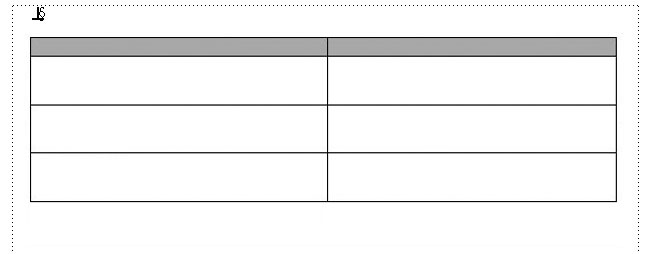
\includegraphics[draft,width=\linewidth]{foo_2col}
    \caption{Significant graph for size-3 motifs}
\end{figure*}

\begin{figure*} \label{fig:sigm4}
    \centering
    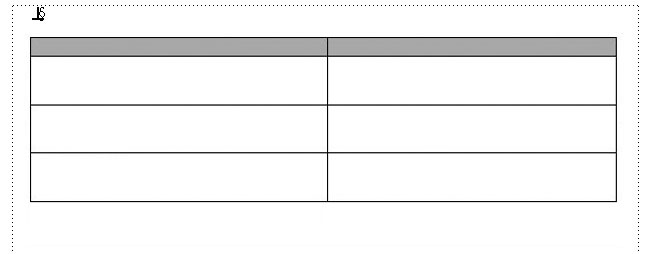
\includegraphics[draft,width=\linewidth]{foo_2col}
    \caption{Significant graph for size-4 motifs}
\end{figure*}

\begin{table}
\centering
\begin{tabular}{c c}
\textsc{Dataset} & \textsc{Motif} \\
\hline \\
\textsc{Blogcatalog} & Figure \ref{fig:m3}-m2 \\
\textsc{PPI} & Figure \ref{fig:m3}-m4 \\
\textsc{Citeseer} & Figure \ref{fig:m4}-m7 \\
\textsc{Cora} & Figure \ref{fig:m4}-m7 \\
\textsc{Pubmed} & Figure \ref{fig:m4}-m7 \\
\textsc{NELL} & Figure \ref{fig:m3}-m4 \\
\end{tabular}%
\caption{Target motifs for each network}
\label{t:motifs}
\end{table}

\section{Results}

We report the performance of each algorithm on graph node
labeling task.

\subsection{Unsupervised node labeling}

\begin{table}[H]
\centering
\resizebox{\columnwidth}{!}{%
\begin{tabular}{c | c c c}
\textbf{\textsc{Method}} & \textsc{BlogCatalog} & \textsc{Citeseer} & \textsc{PPI} \\
\hline \\
Spectral clustering & 0.23 & 0.30 & 0.14  \\
Deepwalk & 0.22 & 0.65 & 0.18 \\
Node2Vec & 0.22 & 0.66 & \textbf{0.18} \\
\textbf{motifwalk} & \textbf{0.24} & \textbf{0.68} & 0.17 \\
\end{tabular}%
}
\caption{F1-macro score for multiclass labeling}
\label{t:re}
\end{table}

\subsection{Semi-supervised node labeling}

\begin{table*}[H]
\centering
\begin{tabular}{c | c c c c}
\textbf{\textsc{Method}} & \textsc{Citeseer} & \textsc{Cora} & \textsc{Pubmed} & \textsc{NELL} \\
\hline \\
Deepwalk & 43.2 & 67.2 & 65.3 & 58.1 \\
\textbf{motifwalk} & 45.7 & 68.0 & 64.9 & 58.8 \\
Planetoid & 64.7 & 75.7 & 77.2 & 61.9 \\
GCN & 70.3 & 81.5 & 79.0 & 66.0 \\
\textbf{m-GCN} & \textbf{71.2} & \textbf{82.1} & \textbf{79.5} & \textbf{66.1} \\
\hline \\
m-GCN (rand. splits) & 70.2 $\pm$ 0.5 & 81.1 $\pm$ 0.5 & 79.3 $\pm$ 0.7 & 62.0 $\pm$ 1.4 \\
\end{tabular}%
\caption{Accuracy score for multiclass labeling}
\label{t:re}
\end{table*}

\section{Related work}

\subsection{Spectral approaches}

\subsection{Skipgram-based approaches }

\subsection{Deep neural network approaches}

\section{Discussion}

Our paper's contributions are proposing an extension to the graph convolutional 
architecture; proposing the uses and demonstrate the importance of motifs in
real worldnetworks.

Limitation: 


\section*{Acknowledgments}

I would like to thank.

%% The file named.bst is a bibliography style file for BibTeX 0.99c
\bibliographystyle{named}
\bibliography{ijcai17}

\end{document}

